% ---------------------------------------------------------------------------
% Author guideline and sample document for EG publication using LaTeX2e input
% D.Fellner, v1.15, Dec 14, 2018

\documentclass{egpubl}
 
% --- for  Annual CONFERENCE
% \ConferenceSubmission   % uncomment for Conference submission
% \ConferencePaper        % uncomment for (final) Conference Paper
% \STAR                   % uncomment for STAR contribution
% \Tutorial               % uncomment for Tutorial contribution
% \ShortPresentation      % uncomment for (final) Short Conference Presentation
% \Areas                  % uncomment for Areas contribution
% \MedicalPrize           % uncomment for Medical Prize contribution
% \Education              % uncomment for Education contribution
% \Poster                 % uncomment for Poster contribution
% \DC                     % uncomment for Doctoral Consortium
%
% --- for  CGF Journal
% \JournalSubmission    % uncomment for submission to Computer Graphics Forum
\JournalPaper         % uncomment for final version of Journal Paper
%
% --- for  CGF Journal: special issue
% \SpecialIssueSubmission    % uncomment for submission to , special issue
% \SpecialIssuePaper         % uncomment for final version of Computer Graphics Forum, special issue
%                          % EuroVis, SGP, Rendering, PG
% --- for  EG Workshop Proceedings
% \WsSubmission      % uncomment for submission to EG Workshop
% \WsPaper           % uncomment for final version of EG Workshop contribution
% \WsSubmissionJoint % for joint events, for example ICAT-EGVE
% \WsPaperJoint      % for joint events, for example ICAT-EGVE
% \Expressive        % for SBIM, CAe, NPAR
% \DigitalHeritagePaper
% \PaperL2P          % for events EG only asks for License to Publish

% --- for EuroVis 
% for full papers use \SpecialIssuePaper
% \STAREurovis   % for EuroVis additional material 
% \EuroVisPoster % for EuroVis additional material 
% \EuroVisShort  % for EuroVis additional material

% !! *please* don't change anything above
% !! unless you REALLY know what you are doing
% ------------------------------------------------------------------------
\usepackage[T1]{fontenc}
\usepackage{dfadobe}  
\usepackage{float}

%\usepackage{cite}  % comment out for biblatex with backend=biber 
% ---------------------------
\biberVersion
\BibtexOrBiblatex
\usepackage[backend=bibtex,bibstyle=EG,citestyle=alphabetic,backref=true]{biblatex} 
\addbibresource{egbibsample.bib}
% ---------------------------  
\electronicVersion
\PrintedOrElectronic

% for including postscript figures
% mind: package option 'draft' will replace PS figure by a filename within a frame
\ifpdf \usepackage[pdftex]{graphicx} \pdfcompresslevel=9
\else \usepackage[dvips]{graphicx} \fi

\usepackage{egweblnk} 
% end of prologue

% ---------------------------------------------------------------------
% EG author guidelines plus sample file for EG publication using LaTeX2e input
% D.Fellner, v2.03, Dec 14, 2018


\title[Evolution of a Star Cluster using Gravitational N-Body Simulations]%
      {Evolution of a Star Cluster using Gravitational N-Body Simulations}

% for anonymous conference submission please enter your SUBMISSION ID
% instead of the author's name (and leave the affiliation blank) !!
% for final version: please provide your *own* ORCID in the brackets following \orcid; see https://orcid.org/ for more details.
\author[S. Walker]
	{Simon Lewis Walker}
% ------------------------------------------------------------------------

% if the Editors-in-Chief have given you the data, you may uncomment
% the following five lines and insert it here
%
% \volume{36}   % the volume in which the issue will be published;
% \issue{1}     % the issue number of the publication
% \pStartPage{1}      % set starting page


%-------------------------------------------------------------------------
\begin{document}

% uncomment for using teaser
% \teaser{
%  
\includegraphics[width=\linewidth]{eg_new}
%  \centering
%   \caption{New EG Logo}
% \label{fig:teaser}
%}

\maketitle
%-------------------------------------------------------------------------
\begin{abstract}
The evolution of a star cluster can be accurately animated by using N-body simulations with the number N of particles limited from 1 to $5\times10^3$. I develop an N-body simulation code on my own personal computer by editing the base code provided by our professor, M. Haworth. I execute different N-body simulations randomizing the starting position and mass of each particle to form unique instances of star clusters. The maximum number of particles that can be simulated on my machine is $5\times10^3$, in which 1 particle corresponds to a star within the star cluster. I find that the randomly generated star clusters end up clumping in the center of the screen where most of the massive particles of the simulation will be.
\end{abstract}  
%-------------------------------------------------------------------------
\section{Introduction}

    N-body simulations have plenty of use being a theoretical tool for scientific and engineering applications. One of these applications uses the gravitational n-body simulation to simulate the creation and evolution of star systems, star clusters, galaxies and galaxy clusters. The difficulty with these problems is calculating the physical equations which govern how everything in the seeable universe interact with each other in real time. It is possible to do smaller amounts of particles but in order to get an accurate representation we must use as many particles as we can to simulate these systems.

%-------------------------------------------------------------------------
\section{Related Work}

%-------------------------------------------------------------------------
\subsection{Cosmological N-Body Simulations}

    Cosmological N-Body Simulations is a paper written by Edmund Bertschinger and James M. Gelb where they discuss the usage of N-body simulations for simulating gravitation forces on a large scale. Specifically, their goal was to see how a system like this would act if they included the dark matter theory. In their experiments they had access to supercomputer hardware and software, so they were able to use $256^3$ particles. They achieved this by using the hierarchical tree or particle-particle/particle mesh algorithms which also helped increase the resolution. Later they used Couchman’s algorithm which made it possible for them to compute this to up to 16.8 million particles. They were able to confirm the self-similarity of gravitational clustering by using the initial conditions they chose. The problem with this is that the conditions are unrealistic in our own universe. What they found should be used as approximations for the real thing.  The gravity instability they found should be used as it found that the dark matter began to clump together looking like galaxy halos. This is important as it will help galaxy formation theories. This paper was written in 1991 where they did not have as powerful computers as we do now so they stated that what they discovered helped, but with the improvement of computers, there will be even better way to simulate the formation of galaxies.

    From this paper I read about a hierarchical tree code which was used in order to deal with the N problem of the N-body simulations. They said, “The Hierarchical tree code reduces the operations count to $O(NlogN)$ by treating distant clumps of particles as single massive pseudo particles” ~\cite{bertschinger1991cosmological} Using this I attempted to implement a similar system within my own code. Regretfully I was unable to complete this portion, but I was able to simulate something similar where I only considered particles within a certain radius. I was able to make the simulation deal with every 200 particles that were near each other. I had to do this manually by creating a function for the force calculation and write it in a way so that it read 200 particles at a time. This did give me an increase in efficiency as I was able to increase the amount of particles I could deal with from 500 to 5000.

%-------------------------------------------------------------------------
\subsection{Visualizing astrophysical N-body systems}

    Visualizing astrophysical N-body systems is a paper written by John Dubinski who discusses case studies that have dealt with N-body simulations that accurately simulate what is in our own universe. He discusses specific cases like cosmological simulations, nightfall animation, and MW-Andromeda collision animation. Through these he points out that the evolution of computer graphics has assisted in creating a visible universe. Originally, most of these visualizations were using dotted figures but now that we have developed new methods, using graphics cards and faster computers, we are able to simulate images and animations that are valuable tools for interpreting and comparing to our visible universe. He notes that these simulations are becoming more and more like the real thing. The next challenge is to create photo realistic animations that would resemble photo taken from the Hubble space telescope. This means the animation would need to include gas, stars and dark matter in the calculation. 

    This paper gives me a great goal to have for where I might take this project. Currently it only simulates stars and does not compute for anything else that might effect it. But with the animations that this paper has shown it has increased my interesting in perhaps trying to do more with it. Many of the images in the paper show these images from the simulations/animations of other projects that were investigation the possibilities of simulating N-body systems. Many of them, like the MW-Andromeda collision which simulates the collision of the MW and Andromeda galaxies, look photo realistic as the two spirals meet and interact with each other~\cite{dubinski2008visualizing}.

%-------------------------------------------------------------------------
\subsection{Particle Number Dependence of the N-body Simulations of Moon Formation}

    Particle Number Dependence of the N-body Simulations of Moon Formation is a paper written by Takanori Sasaki and Natsuki Hosono which discusses the use of N-body simulations to simulate the multiple ways that our moon could have formed ~\cite{sasaki2018particle}. In this simulation they used $10^4$ or $10^7$ particles to simulate where the proto-moon forms, where they found it did so just outside of the Roche limit radius. It created spiral structures from the gravitational instability which causes the angular momentum to enhance from the gravitational torque and the coherent motion of the wakes. They found that depending on the number N in the N-body simulation would give differences in the qualitative and quantitative in the formation of the Moon.

    I used the outcome of this paper to finalize what parameters I should use for my own simulations. Though I used less particles, it still helped me find the sweet spot where the simulation could run smoothly and give an accurate animation. They also used to discuss the methods of their calculations where they sued the equation of motion and found the Roche limit. I was unable to configure the Roche limit within my own animation as it would mean each particle would have to compute this comparing it to each particle nearby. Since I was developing a star cluster this would not have helped in anyway. However, I did end up using the equation of motion in my assignment. Using it to help in figuring out the force each particle has on one another. 

%-------------------------------------------------------------------------
\section{Overview}

    The implementation of this project started off with the example code that was provided to us by Professor Brandon Haworth. Using his work, I was able to not worry about how to get things to be view on screen, but focus specifically on the calculations that I would need to do to get an accurate simulation of star clusters. Originally starting off with very very few stars just to see if they would interact with each other. After I was able to achieve this I went on and decided to try more and more particles into the simulation. As I did I discovered that my code was running in $O(N^2)$ as the animation came to a stutter. In order to fix this problem, I began to read up on the Barnes-Hut tree which takes the space and splits it into separate areas so that you will not have to compare two particles that are extremely far away from each other. This would give a $O(NlogN)$ computation time. I was not able to implement this, so I decided to manually split up my array of stars comparing them in chunks of 200. This made it possible from my original 500 particles to being able to do around 5000.

    The main equation that I used in this simulation is Newtons Law of Universal Gravitation. This equation is the backbone of my entire program as this is how each particle can interact with each other. In this program we need to calculate the force exerted to each particle by each particle. In order to simplify this, I tried to implement my own version of Barnes-Hut tree. It starts by recursively dividing the N bodies into groups and storing those into and Octree where each node of the tree is a region in this space. The top node is the entire space and its eight children are the eight octants of it. This is done for each of those eight octants until we are left with only zero or one bodies for each child. From there you only calculate the force between each particle within each octant. Averaging out the force exerted upon each section of the tree. I was not able to achieve this in my own code but I hope to do so soon. The last equation that needs to be noted is the Equations of Motion that I got from Particle Number Dependence of the N-body Simulations of Moon Formation by Takanori Sasaki and Natsuki Hosono~\cite{sasaki2018particle}. With this I was able to calculate the velocities and accelerations of each of the particles after calculating the force that would be exerted on each of them. From this I began to read about Newtonian Mechanics and Kinematic quantities of which I would have liked to use to possibly make the animation smoother.

%-------------------------------------------------------------------------
\section{Evaluation}

\begin{figure}[H]
  \centering
  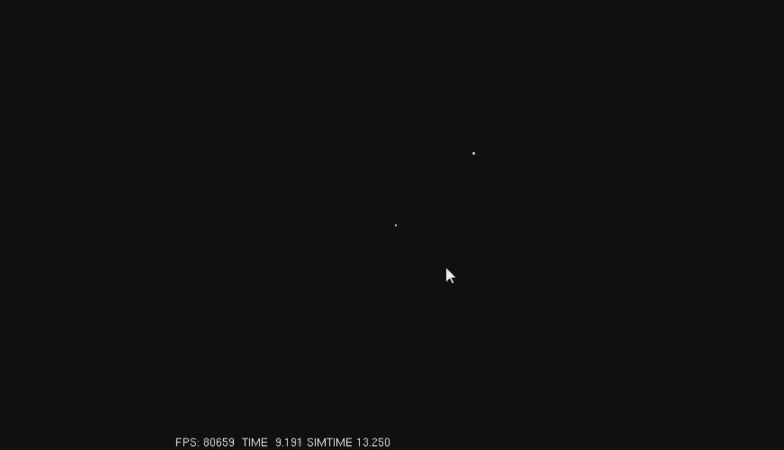
\includegraphics[width=.8\linewidth]{Screen_Caps/001_and_001_1.png}
  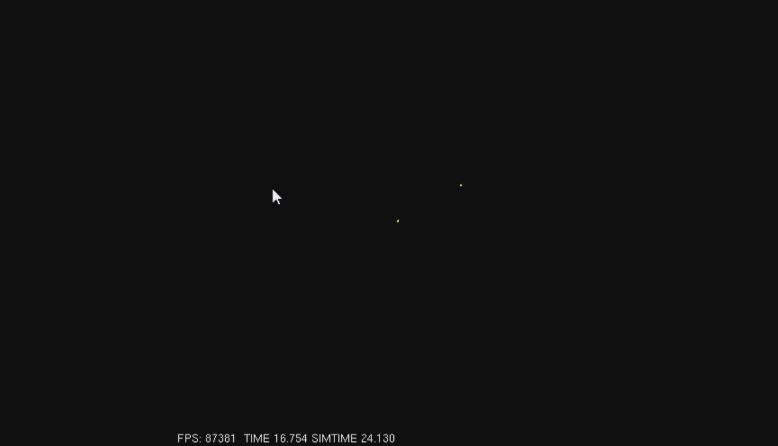
\includegraphics[width=.8\linewidth]{Screen_Caps/001_and_001_2.png}
  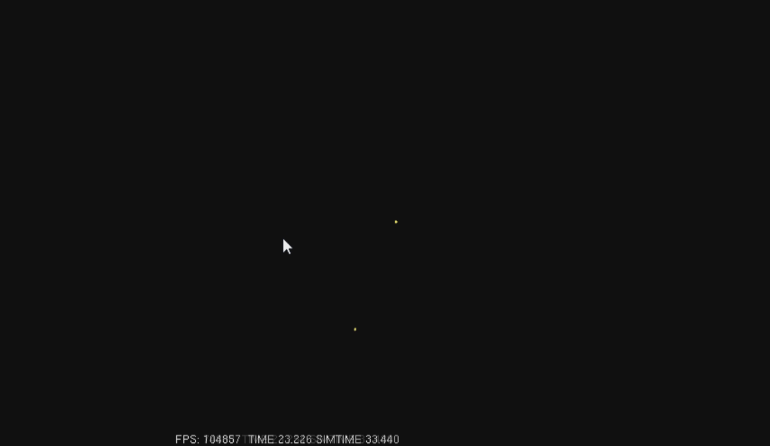
\includegraphics[width=.8\linewidth]{Screen_Caps/001_and_001_3.png}
  \caption{\label{fig:Fig1}
           Simulation of 2 particles before and after passing by each other where the mass of each is set to 0.01.}
\end{figure}

\begin{figure}[H]
  \centering
  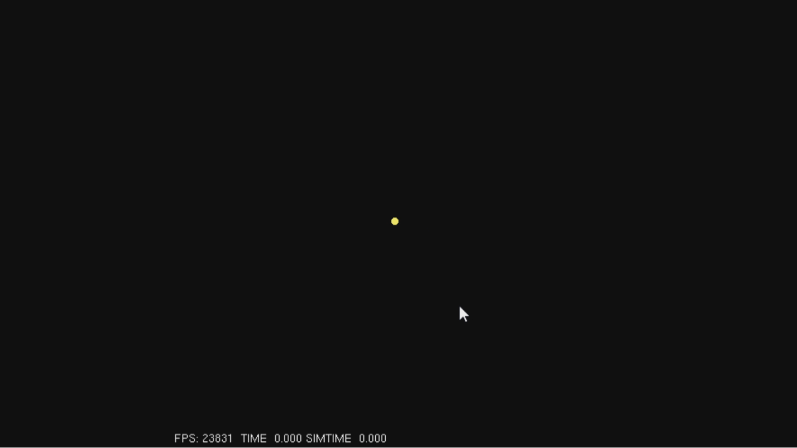
\includegraphics[width=.8\linewidth]{Screen_Caps/500ptk_1000000_and_1_1.png}
  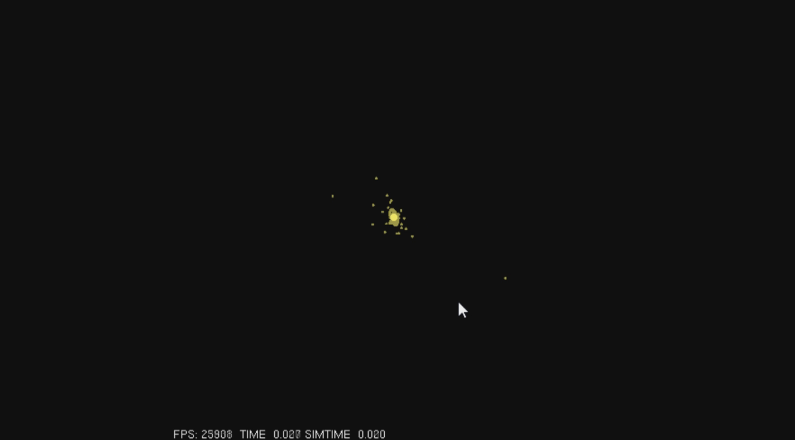
\includegraphics[width=.8\linewidth]{Screen_Caps/500ptk_1000000_and_1_2.png}
  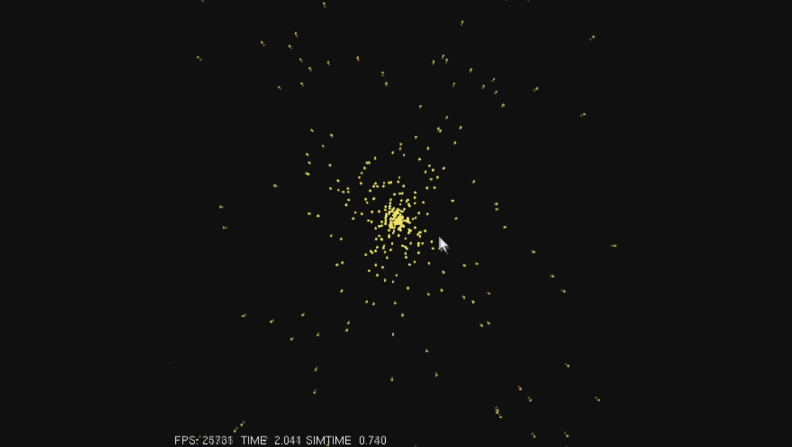
\includegraphics[width=.8\linewidth]{Screen_Caps/500ptk_1000000_and_1_3.png}
  \caption{\label{fig:Fig2}
           Simulation of 500 particles where the center mass is set to 1000000 and the other masses are set to 1.}
\end{figure}

    After finally achieving a runnable program I began by running small number Ns on the N-body simulation. Starting off with 2 to see how they would interact with each other and slowly move up from there. This was on my original code where I could only simulate using 500 particles. This did give reasonable output as each couple of frames it was obvious that the particles were interacting with each other. I used specific positions and masses for the first few runs to see if anything would change. When it didn’t, I moved on to making the positions and masses randomly chosen.

    For the project I used my own person computer to run the simulations. My system has an Intel i7-7740X CPU running at 4.30GHz, 16gb ram running at 2133MHz, and an NVIDIA GeForce GTX 970 with 4.0GB of dedicated GPU memory. I currently ran everything off of the CPU than the GPU as I was unable to figure out how to have the system be simulated using the GPU to do the thousands of computational tasks. 

\begin{figure}[H]
  \centering
  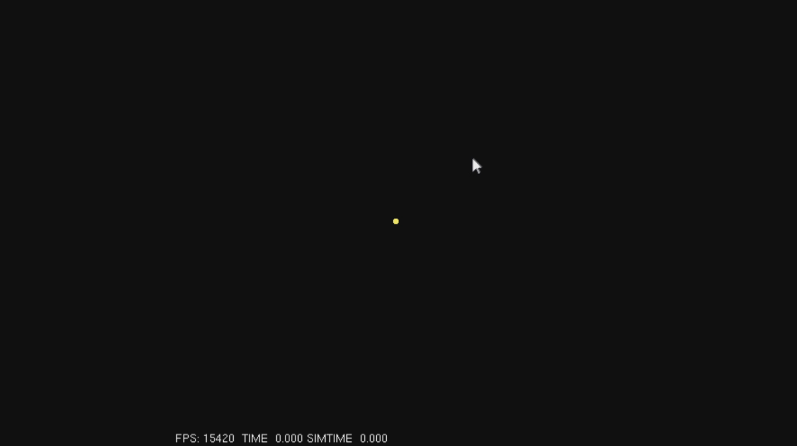
\includegraphics[width=.8\linewidth]{Screen_Caps/1000ptk_10000_and_1_1.png}
  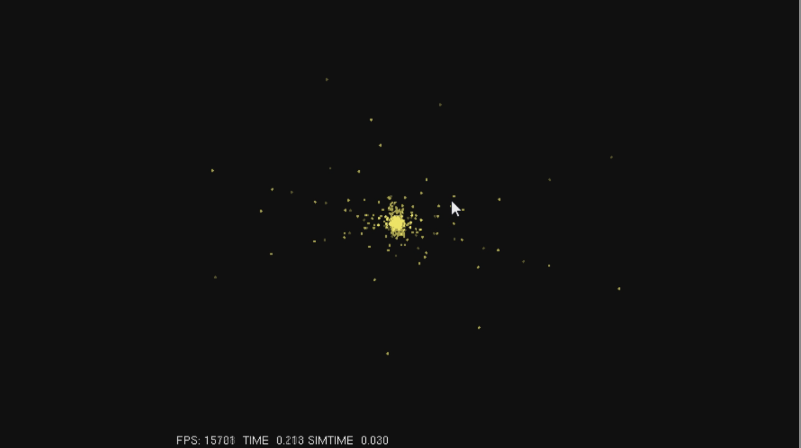
\includegraphics[width=.8\linewidth]{Screen_Caps/1000ptk_10000_and_1_2.png}
  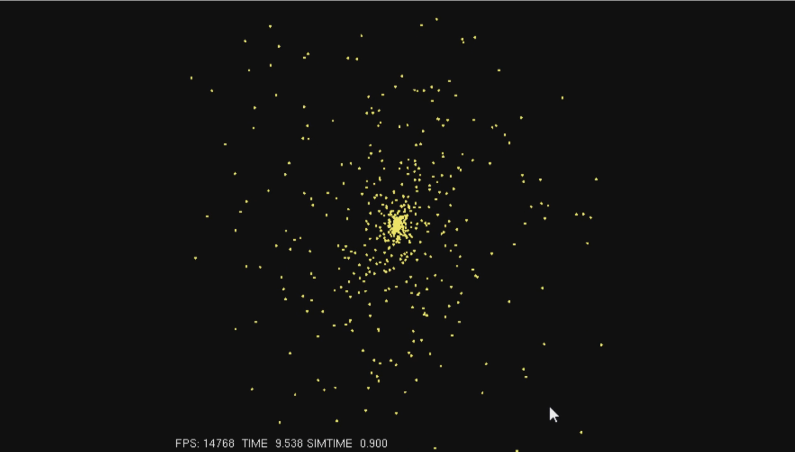
\includegraphics[width=.8\linewidth]{Screen_Caps/1000ptk_10000_and_1_3.png}
  \caption{\label{fig:Fig3}
           Simulation of 1000 particles where the center mass is set to 10000 and the other masses are set to 1.}
\end{figure}

    When I first began simulations I the particles accelerations would always go to infinity which caused me many problems. This meant that something was wrong in my code, so I had to figure out what specifically had gone wrong to fix it. Going through most of it I discovered that most of my math was incorrect. I did more research on the topic discovering Newtons Law of Gravitation and the kenematic equations from the equations of motion which I realized I was not using. Newtons Law of Gravitation is as shown:

Newtons Law of Gravitation: $F = G\times \frac{m_1 \times m_2 }{r^2}$

Where $G = 6067408 \times 10^-11 m^3 kg^-1 s^-2$, $m_1$ and $m_2$ are the two masses, and lastly $r$ is the dsitance between the two masses~\cite{sasaki2018particle}. The equations of motion are as follows:

Kenematic equations for a particle: $v = \frac{dr}{dt}, a = \frac{dv}{dt} = \frac{d^2r}{dt^2}$

Where $r = r(t)$ is position, $t$ is time, $v = v(t)$ is velocity, and $a = a(t)$ is acceleration. After implementing both of those I was able to receive a working system where the particles did interact with each other. The difficult part was trying to get them to look like a normal star system in which I realized was harder than it seemed. I originally had the idea of having out solar system exist. So, planets would be revolving around stars. But in order to do something like that I would need to use the Two-body problem which I was not prepared to implement into my system. Specifically, because I would need to calculate this equation for every particle in the system. I decided against doing this and just calculating the gravitational force that would be exerted upon each particle.

\begin{figure}[H]
  \centering
  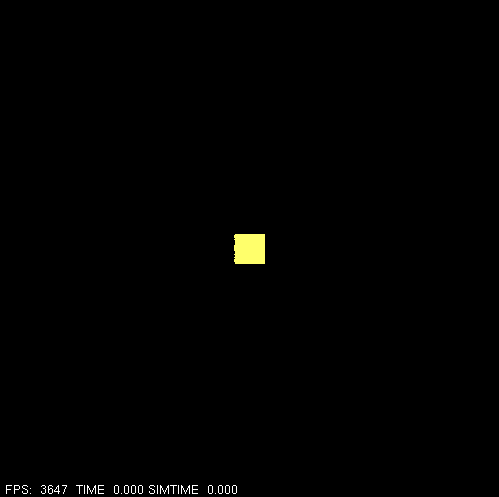
\includegraphics[width=.5\linewidth]{Screen_Caps/5000ptk_100_and_X_1.png}
  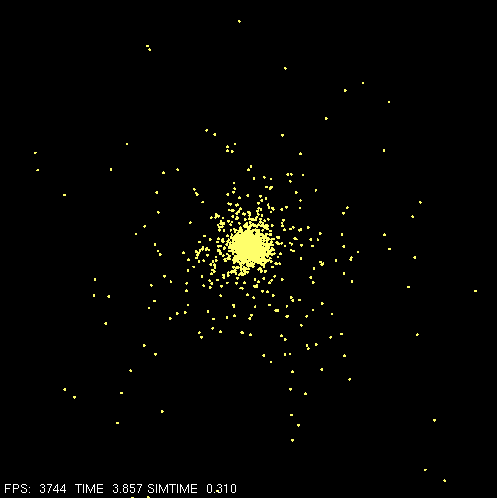
\includegraphics[width=.5\linewidth]{Screen_Caps/5000ptk_100_and_X_2.png}
  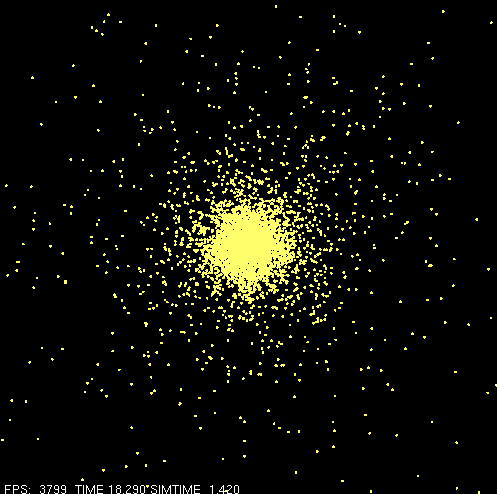
\includegraphics[width=.5\linewidth]{Screen_Caps/5000ptk_100_and_X_3.png}
  \caption{\label{fig:Fig4}
           Simulation of 5000 particles where the center mass is set to 100 and the other masses are set between 100 and 1.}
\end{figure}

\begin{figure}[H]
  \centering
  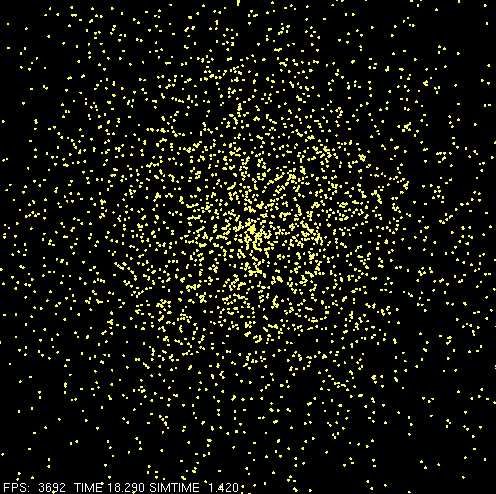
\includegraphics[width=.5\linewidth]{Screen_Caps/5000ptk_100_and_X_4_ZOOM.png}
  \caption{\label{fig:Fig5}
           Closer view of the particles within the cluster from Figure 5.}
\end{figure}

%-------------------------------------------------------------------------
\section{Conclusion}

I have created a way to simulate the evolution of a star cluster by using a gravitational N-body simulation. I was able to accurately simulate the forces of gravity acting upon each particle as the cluster slowly forms. After some difficulty, I achieved to run a simulation using 5000 particles using a similar method like the Barns-Hut tree. This produces an animation that looks like the ones that were being animated on super computers using millions of particles. I knew that I would not be able to make anything as amazing as their work, but I was very excited to see something that looked incredibly like what they had done. The simulations also ran smoothly on my machine in the under 2000 particles. When I started to run when N is equal to 5000 my system started to become restricted. The frame rate dropped, but still ran and produced a reasonable animation of the star cluster. If I had a stronger computer or if I had learned how to use the GPU rather than the CPU to do the calculations, I might have been able to use a larger number for N.

The challenges I faced I felt were simple to find but hard to create reasonable answers for. I started off setting an array to hold all the information of each particle. But this did not account for the possibility of having N particles. So instead I used the ValArray in C++ so that I could resize it to whatever is needed for N. In order to have the system animate and have a reasonable look I had to add some limiting factors. The velocity would occasionally be calculated at being at infinity, so I had to set a parameter to limit the maximum velocity a particle can travel at. I also was having difficulty finding which equations to use in this project. Thinking about how I would be able to calculate the force between each particle I originally thought would just be its mass times its acceleration. This led me to discovering Newtons Law of Universal Gravity, which gave me the constant that I needed in order to solve for the force that each particle will be exerting on each other.

I was really inspired from reading about the work other people have done. Though they had better resources than me, being able to possibly create the animations and images that they did sounds like a great goal to have. I would like to add in a black hole, or at the very least, a gravity well that would destroy the points when they would be pulled in by the gravity. Possibly also giving each particle its own radius and brightness so that when they do form clusters it would be easy to tell whereas you could tell by the collective brightness of each star there. Before all of this I think I would like to try to implement Barnes-Hut trees so that I could possibly do more than 5000 particles. This could potentially give me the visuals that I had looked forward to making since the start of this project. 

Overall, this project was really eye opening for and has really helped me think more about my goals of being a Computer Scientist in the field of graphics and gaming. Learning about all these styles and methods has really shown that this is not an easy thing to accomplish. So, I am thankful that I was able to get this far with it.


%-------------------------------------------------------------------------
\printbibliography[heading=bibnumbered]


\end{document}
